\documentclass{beamer}
%使用主题
\usetheme{CambridgeUS}
%\usefonttheme[stillsansseriftext,stillsansserifsmall,stillsansseriflarge]{serif}
\usefonttheme[onlymath]{serif}
\usepackage[fontset=fandol]{ctex}
\setCJKsansfont{FandolSong}
%\usepackage{fancyvrb}
\usepackage{amsmath,amssymb}
\usepackage{amsthm}
\usepackage{tikz}
\usepackage{booktabs}
\usepackage{graphicx}
\usepackage{multicol}
\usepackage{enumerate}
\usepackage{siunitx}
\usepackage{hyperref}
\hypersetup{colorlinks,%
            linkcolor=blue,%
            bookmarksopen=true}
        
%%%必须参数和可选参数
\newcommand\m[1]{\mbox{$\langle${\rmfamily\textit{#1}\/}$\rangle$}}
\newcommand{\marg}[1]{{\tt\string{}\m{#1}{\tt\string}}}
\newcommand{\oarg}[1]{{\tt[}\m{#1}{\tt]}}
%\logo{This is a logo}

%\setbeamercovered{transparent}

\begin{document}

\begin{frame}
\title{使用Beamer文档类制作演示文档\thanks{\LaTeX{} in 24 hours(Dilip Datta) and Beameruserguide}}
\subtitle{一个有用且强大的工具}
\author{Swit}
\institute{School of Mathematics and Statistics\\
Wuhan University\\WuHan}
\date{March 10,2020}
\maketitle
\end{frame}

\begin{frame}
\begin{multicols}{2}
\tableofcontents
\end{multicols}
\end{frame}

\section{概述}
\begin{frame}
\frametitle{概述}
Beamer文档类是专用于制作演示文稿的\LaTeX{} 文档类,本文只是对此文档类的一些粗略介绍,如果需要全面深入地了解Beamer文档类请查阅Till教授所著的Beameruserguide,此文档可在ctan官网获取 \url{http://mirrors.ctan.org/macros/latex/contrib/beamer/doc/beameruserguide.pdf} 或者直接通过命令行工具texdoc获取。
\end{frame}

\section{帧(Frame)}
\subsection{帧的创建}
\begin{frame}[containsverbatim]
\frametitle{帧}
%In the document-class beamer, a presentation consists of a number of frames. A frame is created by two means:
在Beamer文档类中,一个演示文档由一系列帧组成,每一帧由一系列幻灯片(slide)组成。每一帧通过两种方式创建:
%\begin{itemize}
%\item Command:\verb|\frame[][]{}|
%\item %Environment:\verb|\begin{frame}[][]...\end{frame}|
%\end{itemize}
\begin{itemize}
\item 命令:\verb|\frame[][]{}|
\item 环境:\verb|\begin{frame}[][]...\end{frame}|
\end{itemize}
每一帧的内容写在命令 \verb|\frame[][]{}| 的必选参数中或者环境 \verb|frame| 之中。
\end{frame}


\subsection{帧的组成部分}
\begin{frame}[allowframebreaks,containsverbatim]
\frametitle{帧}
\framesubtitle{帧的组成部分}
%A frame generally consists of some or all of the following eight components:(according to the theme you choose)
每一帧由下列八个组成部分的一部分或者全部所构成(根据你选择的主题而定):
%\begin{enumerate}
%\item Headline and footline
%\item Sidebars: Sidebars are generated automatically by the chosen theme on either
%side for displaying mainly the table of contents of %the presentation.
%\item Navigation bar
%\item Navigation symbols(slide icon,frame icon,subsection icon,section icon,presentation icon,appendix icon,back and forward icons,search icon)
%\item Logo:\verb|\logo{}|
%\item Frame title:A title and a subtitle can be assigned to a frame using the \verb|\frametitle{}|
%and \verb|\framesubtitle{}|
%\item Background
%\item Frame contents:By default the contents of a frame (except the title and subtitle) are
%vertically center aligned. This
%default alignment can be changed by the options t for top alignment, c(default)
%for vertically center alignment and b for bottom alignment. A vertical alignment option may be assigned to \verb|\documentclass[]{beamer}| for global effect in all
%frames. Alternatively, it can be used as an option to a particular frame for local
%effect only, e.g., \verb|\frame[t]{}| or \verb|\begin{frame}[t]|.
%\end{enumerate}
\begin{enumerate}
	\item 顶部导航区(Headline)和底部导航区(Footline)
	\item 侧边栏(Sidebars):由选择的主题自动生成并置于帧的一侧主要用于展示演示文档的目录。
	\item 导航条(Navigation bar):导航栏也是由选择的主题自动生成的,主要用于下面两个目的:
	\begin{enumerate}
		\item 为观众提供视觉反馈,让其知道演示文档隐藏了多少以及将要指向何处。
		\item 可以点击导航条的任意部分实现目标位置跳转。
	\end{enumerate}
	\item 导航图标(Navigation symbols):每一张幻灯片的右下角都有浅灰色的小型导航图标,它们从左到右分别为幻灯片图标、帧图标、子节图标、节图标、演示稿图标、附录图标(存在附录时才显示该图标)、返回图标与前进图标、搜索图标。
	\item 徽标(Logo):可以在导言区使用 \verb|\logo{}| 命令进行徽标的全局插入,\verb|\logo{}| 命令的参数可为文本或图片插入命令。Logo插入的位置由主题判定。
	\item 帧标题(Frametitle):使用 \verb|\frametitle{}| 命令和 \verb|\framesubtitle{}| 命令分别添加帧标题和帧副标题。
	\item 背景(Background):每一帧都有一个背景,背景由背景画布(Background canvas)和主背景(Main background)组成。
	\item 内容(Frame contents):帧的内容可以是普通的 \LaTeX{} 文本,但是不可以包含 \verb|\verb| 命令或者 \verb|\verbatim| 环境\footnote{解决此问题有三个办法:(i)为frame环境添加fragile选项(ii)为frame环境添加containsverbatim选项(iii)在frame环境中使用semiverbatim环境},也不能包含能改变字符代码的任意环境,否则必须加上 \verb|fragile| 选项。
\end{enumerate}
\end{frame}

%\section{Sectional Units in Presentation}
\section{节单元}
\begin{frame}[containsverbatim]
%\frametitle{Sectional Units in Presentation}
\frametitle{演示文档的节单元}
%The frames of a presentation, may be put under various sections
%and subsections produced through \verb|\section[]{}| and \verb|\subsection[]{}|. Unlike in standard
%\LaTeX, \verb|\section[]{}| and \verb|\subsection[]{}| here do not create any heading at their positions, rather they add entries in the table of contents and navigation bars. 
我们可以使用 \verb|\section[]{}| 命令和 \verb|\subsection[]{}| 命令来组织文档,不像标准 \LaTeX{},这些命令不会在用它们的地方创建标题。相反,它们会添加条目到目录和导航条中。

\begin{block}{命令}
\verb|\section|\oarg{short section name}\marg{section name}
\end{block}
当不指定可选参数时,在目录和导航条中都会显示 \m{section name},当指定可选参数 \m{short section name}时,导航条中会替换为 \m{short section name}。
\end{frame}

%\section{Presentation Structure}
\section{演示文档的结构}
\begin{frame}[containsverbatim]
%\frametitle{Presentation Structure}
\frametitle{演示文档的结构}
一个演示文档主要包含下面几个方面的内容:
\begin{itemize}
\item 标题页(Title page)
\begin{itemize}
\item 标题与副标题(Title and subtitle):\verb|\title[]{},\subtitle{}|
\item 作者(Author):\verb|\author[]{}|
\item 所属机构(Institute):\verb|\institute[]{}|
\item 日期(Date):\verb|\date{}|
\item 标题页Logo(Logo in titlepage):\verb|\titlegraphic{}|
\end{itemize}
\item 目录(Table of contents)
\item 主体内容(Presentation materials)
\item 附录(Appendix)
\item 参考文献(Bibliography)
\item 致谢词(Thanks giving)
\end{itemize}
\end{frame}

%\section{Beamer Themes}
\section{Beamer主题}
\begin{frame}[fragile]
%\frametitle{Beamer Themes}
\frametitle{Beamer主题}
%The appearance of a presentation in the beamer document-class can be controlled by five types of themes, which are \textcolor{blue}{presentation theme, color theme, font theme, inner theme,
%and outer theme}.\\
演示文档的外观由五种主题进行控制,它们分别是:演示主题(Presentation theme)、颜色主题(Color theme)、字体主题(Font theme)、内部主题(Inner theme)以及外部主题(Outer theme)。
%A presentation theme generally controls every single detail of the
%appearance of a presentation. Since every presentation theme uses a default set of
%other four themes, normally no other theme is required to be specified if a presentation
%theme is chosen. In order to alter the default setting of a presentation theme, still
%separate color, font, inner, or outer theme may be used as per requirement or choice.
一般来说,演示主题控制着演示文档外观的每一个细节。因为每一个演示主题对于其它四个主题都有一套默认的使用方式,所以当选定了演示主题之后,我们一般无需再去选定其它四个主题。使用五种主题的命令分别为:
\begin{block}{修改主题的命令}
\verb|\usetheme|\oarg{options}\marg{name list}
\verb|\usecolortheme|\oarg{options}\marg{name list}
\verb|\usefonttheme|\oarg{options}\marg{name}
\verb|\useinnertheme|\oarg{options}\marg{name}
\verb|\useoutertheme|\oarg{options}\marg{name}
\end{block}
\end{frame}

%\subsection{Presentation Theme}
\subsection{演示主题}
\begin{frame}[allowframebreaks]
%\frametitle{Beamer Themes}
\frametitle{Beamer主题}
%\framesubtitle{Presentation Theme}
\framesubtitle{演示主题}
提尔·坦图(Till Tantau)教授想尽了一切办法如何命名一个主题。他决定用不同的约定俗成的名字来代替累赘的名字:除两种特殊的情况外,所有演示主题均按城市命名。在这些城市中或其附近举办过他或他的合作者参加过的讨论会或研讨会\footnote{关于每个主题的详细信息请参阅Bermeruserguide}。
\begin{enumerate}[I]
\item 无导航条(Without navigation bars)
\begin{enumerate}
\item default 
\item boxes 
\item Bergen(卑尔根市)
\item Boadilla(博阿迪利亚)
\item Madrid(马德里)
\item AnnArbor(安娜堡)
\item CambridgeUS(坎布里奇US)
\item EastLansing(东兰辛)
\item Pittsburgh(匹兹堡)
\item Rochester(罗切斯特)
\end{enumerate}
\item 顶部含树状导航条(With a tree like navigation bar)
\begin{enumerate}
\item Antibes(安提贝)
\item JuanLesPins(瑞昂莱潘)
\item Montpellier(蒙彼利埃)
\end{enumerate}
\item 含目录侧边栏(With a table of contents sidebar)
\begin{enumerate}
\item Berkeley(伯克利)
\item PaloAlto(帕罗奥多)
\item Goettingen(哥廷根)
\item Marburg(马尔堡)
\item Hannover(汉诺威)
\end{enumerate}
\item 含微帧导航(With a mini frame navigation)
\begin{enumerate}
\item Berlin(柏林)
\item Ilmenau(伊尔姆瑙理)
\item Dresden(德累斯顿)
\item Darmstadt(达姆施塔特)
\item Frankfurt(法兰克福)
\item Singapore(新加坡)
\item Szeged(赛格德)
\end{enumerate}
\item 含节与小节列表(With section and subsection tables)
\begin{enumerate}
\item Copenhagen(哥本哈根)
\item Luebeck(吕贝克)
\item Malmoe(马尔摩)
\item Warsaw(华沙)
\end{enumerate}
\end{enumerate}
\end{frame}

%\subsection{Color Theme}
\subsection{颜色主题}
\begin{frame}[allowframebreaks,containsverbatim]
%\frametitle{Beamer Theme}
%\framesubtitle{Color Theme}
\frametitle{Beamer主题}
\framesubtitle{颜色主题}
\begin{enumerate}[I]
%\item Default and special-purpose color
\item 默认和专用的颜色主题
\begin{enumerate}
%\item default: Uses a little special colors and even less backgrounds.
\item default:使用少量特定的颜色和更少的背景。
%\item sidebartab: Changes colors in sidebars in a way that the current entry in the table of contents is highlighted by a different background.
\item sidebartab:该主题会改变侧栏中目录的当前条目的颜色,通过显示该条目后的不同的背景以使该条目高亮显示。
\item structure: Offers a convenient way of changing the color of the foreground structure. Various
options available to the theme include \verb|rgb={r,g,b}| with r, g and b as the decimal
values of red, green and blue between 0 and 1, e.g., \verb|rgb={0.5,0.2,1}|; \verb|RGB={r,g,b}| same with rgb, except the numbers ranging between 0 and 255, e.g., \verb|RGB={120,0,70}|; \verb|cmyk={c,m,y,k}| with c, m, y and k as the values of cyan, magenta, yellow and black between 0 and 1, e.g., \verb|cmyk={1,0,0.3,0.5}|;\verb|cmy={c,m,y}| same with cmyk without any black component; \verb|hsb={h,s,b}| with h, s and b as the values of hue, saturation and brightness between 0 and 1, e.g., \verb|hsb={0.2,1,0.5}|; and \verb|named={cname}| with cname as the name of a predefined color.
\end{enumerate}
\item Complete color
\begin{enumerate}
\item albatross: Uses yellow on blue as the main colors, and also a slightly darker background for blocks(this background can be removed by additionally loading the lily color theme). The \verb|overlystylish| option may be used to this theme for obtaining a background canvas.(Bad looking)
\item beetle: Uses white and black texts on gray background (white text is used for special emphasis
and black text for normal cases). The outer stuff, like the headline/footline, however,
uses a bluish(浅蓝色的) color.(Bad looking)
\item crane: Uses the colors of Lufthansa, whose logo is a crane.
\item dove: It is nearly black and white, which uses grayscale in certain unavoidable cases, but
never a color. It also produces alerted texts in boldface fonts.
\item fly: It is similar to the beetle theme, and uses white/black/gray throughout.
\item monarca: It is based on the colors of the Monarch butterfly(帝王蝶).
\item seagull: Extensively uses different shades of gray color.
\item wolverine: It is based on the colors of the University of Michigan’s mascot, a wolverine.
\item beaver: It is based on the colors of MIT’s mascot, a beaver.
\item spruce: It is based on the colors of the Michigan State University.
\end{enumerate}
\end{enumerate}
\end{frame}

%\subsection{Font Theme}
\subsection{字体主题}
\begin{frame}[allowframebreaks,containsverbatim]
%\frametitle{Beamer Theme}
\frametitle{Beamer主题}
%\framesubtitle{Font Theme}
\framesubtitle{字体主题}
\begin{enumerate}[I]
%\item default: Uses sans serif(无衬线字体) fonts for alenumerateenumeratef the presentation.
\item default:演示文档的所有文本使用无衬线字体(sans serif fonts)
%\item serif: Uses default serif fonts for all texts of the presentation. Some options may also be used, such as \verb|stillsansserifmath| along with the \verb|stillsansseriftext| option for producing mathematical texts in sans serif fonts; \verb|stillsansserifsmall| for producing “small” texts in sans serif fonts, particularly the texts in headline, footline and sidebars; \verb|stillsansseriflarge| for “large” texts in sans serif fonts, like the presentation or frame title; \verb|stillsansseriftext| for normal texts in sans serif fonts; and \verb|onlymath| for mathematical texts in serif fonts.
\item serif:演示文档的所有文本使用衬线字体(serif fonts)。支持下列 \m{options}:
\begin{enumerate}
	\item \verb|stillsansserifmath|:使用无衬线字体排版数学文本。最好同时使用下面的 \verb|stillsansseriftext| 选项,否则在衬线字体中使用无衬线数学文本显得很难看。
	\item \verb|stillsansserifsmall|:使用无衬线字体排版“小”文本,例如,顶部导航区、底部导航区及侧边栏这些地方的文本。
	\item \verb|stillsansseriflarge|:使用无衬线字体排版“大”文本,例如,演示文档标题和帧标题。
	\item \verb|stillsansseriftext|:使用无衬线字体排版普通文本(即上述三种文本以外的文本)
	\item \verb|onlymath|:只用衬线字体排版数学文本。
\end{enumerate}
%\item structurebold: Titles and texts in headline, footline and sidebars are produced in boldface fonts.
%The options that may be used in this theme are \verb|onlysmall| for producing ``small'' texts in headline, footline and sidebars (but not titles) in boldface fonts; and \verb|onlylarge| for producing “large” texts in boldface fonts, particularly in the main title, frame titles, and section entries in the table of contents.
\item structurebold(结构粗体):使用粗体排版标题以及顶部导航区、底部导航区和侧边栏中的文本。支持下列 \m{options}:
\begin{enumerate}
	\item \verb|onlysmall|:使用粗体排版“小”文本,例如顶部导航区、底部导航区和侧边栏中的文本。
	\item \verb|onlylarge|:使用粗体排版“大”文本,例如主标题、帧标题以及目录中的节条目。
\end{enumerate}
\item structureitalicserif(结构斜体衬线): %
%Similar to the structurebold font theme, except texts are produced by serif fonts in boldface and italics modes. The options of the structurebold theme are supported by this theme also.
该主题和 \verb|structurebold| 字体主题相似,但 \verb|structurebold| 字体主题将文本排版成粗体(bold),而该字体主题用标准的衬线字体将文本排版成斜体。该主题支持的 \m{options} 和 \verb|structurebold| 字体主题相同。
\item structuresmallcapsserif(结构小型大写衬线):该主题和 \verb|structurebold| 字体主题相似,但是该主题使用小型大写和衬线字体。该主题支持的 \m{options} 和 \verb|structurebold| 字体主题相同。
\end{enumerate}
\end{frame}

\subsection{内部主题}
\begin{frame}
\frametitle{Beamer 主题}
\framesubtitle{内部主题}
内部主题控制着这些元素的外观:标题和部分页面、itemize环境、enumerate环境、description环境、块环境、定理和证明环境、图和表、脚注以及参考书目条目。
\begin{itemize}
\item default: An item in the itemize environment start with a little triangle.
\item circles: An item in the itemize and enumerate environments, as well as an entry in the table of contents starts with a small circle.
\item rectangles: An item in the itemize and enumerate environments, as well as an entry in the table of contents starts with a small rectangle.
\item rounded: An item in the itemize and enumerate environments, as well as an entry in the table of contents starts with a small ball. The shadow option may be used to add a shadow to all the blocks.
\item inmargin: A block title or item marking is shown on the left side and its body on the right side.
\end{itemize}
\end{frame}

\subsection{外部主题}
\begin{frame}[t,allowframebreaks,containsverbatim]
\frametitle{Beamer主题}
\framesubtitle{外部主题}
外部主题控制着这些元素的外观:顶部导航区、底部导航区、侧边栏、Logo以及帧标题。也就是说,外部主题大概控制着帧的全部布局。
\begin{itemize}
\item default: There is no headline/footline, and the frame title is left flushed.
\item infolines: Headline shows the current section and subsection, while footline shows the author, institution, presentation title, date, and frame count.
\item miniframes
\item smoothbars
\item sidebar
\item split
\item shadow
\item tree
\item smoothtree
\end{itemize}
\end{frame}

\section{Beamer文档类中的环境}
\begin{frame}[allowframebreaks,containsverbatim]
\frametitle{Beamer文档类中的环境}
\begin{enumerate}[I]
\item 块环境
\begin{enumerate}
\item block: \verb|\begin{block}|\marg{title}\verb|...\end{block}|
\item alertblock: \verb|\begin{alertblock}|\marg{title}\verb|...\end{alertblock}|
\item exampleblock: \verb|\begin{exampleblock}|\marg{title}\verb|...\end{exampleblock}|
\end{enumerate}
\item 定理环境:下面的环境没有强制参数,但是可以提供可选参数作为附加标题。除了proof环境之外,其它环境一般在默认标题后面以圆括号包裹附加标题。在proof环境中,可选标题将替代默认标题“Proof”。
\begin{enumerate}
\item theorem
\item definition
\item definitions
\item corollary
\item proof
\item example
\item examples
\item fact
\end{enumerate}
\end{enumerate}
\end{frame}

\begin{frame}
\frametitle{环境演示}
\begin{block}{块标题}
这是一个块环境。
\end{block}
\begin{alertblock}{警示块标题} 
这是一个警示块环境。
\end{alertblock}
\begin{exampleblock}{示例块标题}
这是一个示例块环境。
\end{exampleblock}
\begin{theorem}[正弦定理]
在三角形$ABC$中,我们有如下定理:$\frac{a}{\sin A}=\frac{b}{\sin B}=\frac{c}{\sin C}$。
\end{theorem}
\begin{proof}
分三角形为锐角三角形、直角三角形、钝角三角形直接证明。
\end{proof}
\end{frame}

\section{帧的定制}
\subsection{Logo}
\begin{frame}[containsverbatim]
\frametitle{帧的定制}
\framesubtitle{Logo}
标题页的徽标通过命令 \verb|\titlegraphic{}| 生成,全局徽标通过 \verb|\logo{}| 生成,徽标插入的位置由选择的主题而定。
\end{frame}

\subsection{帧尺寸}
\begin{frame}[containsverbatim]
\frametitle{帧的定制}
\framesubtitle{帧尺寸}
帧的默认尺寸为 \SI{128}{\milli\metre}$\times$\SI{96}{\milli\metre},其长宽比为$4:3$。默认尺寸可以通过 \verb|aspectratio| 选项由下述方式修改: \verb|\documentclass[aspectratio=aval]{beamer}|,其中 \verb|aval| 是长宽比的选择值。详细数据见下表。
\end{frame}
\begin{frame}
\begin{table}
\begin{tabular}{ccc}
\toprule
选择值 & 长宽比 & 帧尺寸\\
\midrule
1610   & 16:10  & \SI{160}{\milli\metre}$\times$\SI{100}{\milli\metre}\\
\midrule
169    & 16:9   & \SI{160}{\milli\metre}$\times$\SI{90}{\milli\metre}\\
\midrule
149    & 14:9   & 140mm$\times$90mm\\
\midrule
141    & 1.41:1 & 148.5mm$\times$105mm\\
\midrule
54     & 5:4    & 125mm$\times$100mm\\
\midrule
43     & 4:3    & 128mm$\times$96mm(default)\\
\midrule
32     & 3:2    &135mm$\times$90mm\\
\bottomrule
\end{tabular}
\caption{帧尺寸选择值表}
\end{table}
\end{frame}

\subsection{Frame Shrinking(收缩)}
\begin{frame}[containsverbatim]
\frametitle{帧的定制}
\framesubtitle{Frame Shrinking}
The \verb|squeeze| option reduces the vertical space between the enumerated and itemized items to zero. The \verb|shrink| option shrinks the texts of a frame by the specified percentage. For example, a frame may be created as \verb|\frame[squeeze]{}| or
\verb|\begin{frame}[squeeze]| for eliminating vertical space between enumerated and itemized items, or as \verb|\frame[shrink=5]{}| or \verb|\begin{frame}[shrink=5]| for shrinking all texts of the frame by 5$\%$.
\end{frame}

\subsection{Frame Breaking}
\begin{frame}[containsverbatim]
\frametitle{Frame Customization}
\framesubtitle{Frame Breaking}
The \verb|allowframebreaks| option may be used in the frame (i.e., as \verb|\frame[allowframebreaks]{}| or \verb|\begin{frame}[allowframebreaks]|), which instructs to display the entire textual contents of a frame by allowing to break it into multiple slides, if required. In that case, the slides will be numbered by appending the frame title as I, II,…. Further, the \verb|allowdisplaybreaks| option (i.e., as \verb|\frame[allowframebreaks, allowdisplaybreaks]{}| or \verb|\begin{frame}[allowframebreaks, allowdisplaybreaks]|) may also be used if a long array of equations is to be split over multiple slides.
\end{frame}

\section{Mathematics In Beamer}
\begin{frame}[allowframebreaks]
\frametitle{Mathematics In Beamer}
在 Beamer 文档类中排印数学公式并无什么特别之处。
\begin{theorem}[Wallice公式]
Consider the integral $\displaystyle I_n=\int_0^{\frac{\pi}{2}}\sin^nx\;\mathrm{d}x$, we can obtain the Wallice formula:
\[\prod_{n=1}^{\infty}\left(1-\frac{1}{(2n)^2}\right)=\frac{2}{\pi}\]
\end{theorem}
\end{frame}

\section{图表}
\begin{frame}[containsverbatim]
\frametitle{图表}
我们可以像平常一样使用标准的 \LaTeX{} figure 和 table 环境。然而,会忽略任何放置规则。在 figure 和 table 环境开始处会立即插入图(Figures)和表(Tables)。如果图表太多在帧中容不下时,必须手工分开它们并将它们放置于不同的帧,或使用 \verb|allowframebreaks| 选项。
\end{frame}

\begin{frame}[t,containsverbatim,allowframebreaks]
\frametitle{图表}
\framesubtitle{Tikz绘图}
\begin{figure}
\flushleft
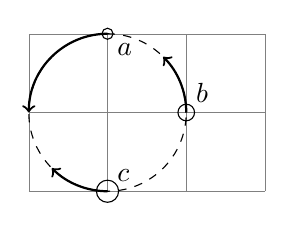
\begin{tikzpicture}
\draw[help lines] (0,0) grid (3,2);
\draw[dashed] (1,1) circle (1cm);
\draw (1,2) coordinate(a) circle (2pt)
      (2,1) coordinate(b) circle (3pt)
      (1,0) coordinate(c) circle (4pt);
\draw[->,thick] (a) arc (90:180:1cm);
\draw[->,thick] (b) arc (0:45:1cm);
\draw[->,thick] (c) arc (270:225:1cm);
\draw (a) node[anchor=north west] {$a$}
      (b) node[anchor=south west] {$b$}
      (c) node[anchor=south west] {$c$};
\end{tikzpicture}
\end{figure}
\begin{verbatim}
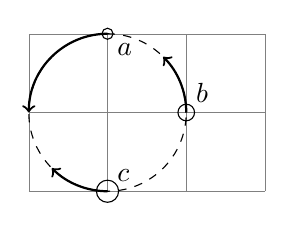
\begin{tikzpicture}
\draw[help lines] (0,0) grid (3,2);
\draw[dashed] (1,1) circle (1cm);
\draw (1,2) coordinate(a) circle (2pt)
      (2,1) coordinate(b) circle (3pt)
      (1,0) coordinate(c) circle (4pt);
\draw[->,thick] (a) arc (90:180:1cm);
\draw[->,thick] (b) arc (0:45:1cm);
\draw[->,thick] (c) arc (270:225:1cm);
\draw (a) node[anchor=north west] {$a$}
      (b) node[anchor=south west] {$b$}
      (c) node[anchor=south west] {$c$};
\end{tikzpicture}
\end{verbatim}
\end{frame}
\end{document}
